\documentclass[11pt,a4paper]{report}

% ---------- packages ----------
\usepackage[margin=1in]{geometry}
\usepackage{graphicx}
\usepackage{amsmath,amssymb}
\usepackage{booktabs}
\usepackage{tabularx}
\newcolumntype{R}{>{\raggedright\arraybackslash}X}
\usepackage{xcolor}
\usepackage{caption}
\usepackage{subcaption}
\usepackage{natbib}
\usepackage[hidelinks]{hyperref}

\graphicspath{{figures/}}

% Placeholder marker for values to be filled from the final training run.
\newcommand{\todo}[1]{\textcolor{red}{[#1]}}

% ---------- title ----------
\title{\bfseries Automated Segmentation of Glioblastoma Sub-regions\\
in Multi-parametric Brain MRI using a 3D U-Net}
\author{Utkarsh Maurya}
\date{September 2026}

\begin{document}

\maketitle

\begin{abstract}
\noindent
Glioblastoma is the most aggressive primary brain tumour in adults, and accurate
delineation of its sub-regions in magnetic resonance imaging (MRI) is essential
for diagnosis, treatment planning and monitoring. Manual segmentation is slow,
labour-intensive and subject to inter-rater variability. This project develops a
fully automated deep-learning pipeline that segments glioblastoma sub-regions
from multi-parametric MRI. Using the BraTS~2020 dataset, we train a
three-dimensional U-Net on the 293 high-grade-glioma (glioblastoma) cases, taking
the four co-registered modalities (T1, T1Gd, T2, FLAIR) as input and producing a
voxel-wise segmentation into background, necrotic/non-enhancing core, peritumoral
edema and enhancing tumour. The network is optimised with a combined Dice and
cross-entropy loss and evaluated with the Dice similarity coefficient and the
95th-percentile Hausdorff distance. On a held-out validation split the model
attains a mean foreground Dice of 0.71 $\pm$ 0.17 across subjects (edema 0.77,
enhancing tumour 0.73, necrotic/non-enhancing core 0.61; per-subject range
0.22--0.94) and localises the tumour reliably, reaching a whole-tumour overlap
(Dice 0.88) competitive with top BraTS~2020 challenge entries despite a far
smaller training budget. We discuss the behaviour of the model across
sub-regions, its per-subject variability, failure cases and limitations, and
describe a deployed interactive web application for tumour detection and
localisation.
\end{abstract}

\tableofcontents

\chapter{Introduction}
\label{ch:introduction}

\section{Motivation}

Gliomas are the most common primary tumours of the central nervous system, and
glioblastoma (GBM, WHO grade~IV) is their most aggressive and most frequent
malignant form in adults. Despite advances in surgery, radiotherapy and
chemotherapy, the prognosis remains poor, with a median survival on the order of
only 12--15 months after diagnosis. Because glioblastoma is highly infiltrative
and heterogeneous, its early and precise characterisation is directly relevant to
treatment planning, surgical guidance, radiotherapy target definition and the
monitoring of disease progression.

Magnetic resonance imaging (MRI) is the primary modality for assessing brain
tumours because it provides excellent soft-tissue contrast without ionising
radiation. In clinical practice several complementary sequences are acquired: a
native T1-weighted scan (T1), a contrast-enhanced (gadolinium) T1-weighted scan
(T1Gd), a T2-weighted scan (T2) and a T2 fluid-attenuated inversion-recovery scan
(FLAIR). Each sequence highlights different tissue properties: the enhancing
tumour rim is most visible on T1Gd, while peritumoral edema and infiltration are
best appreciated on T2 and FLAIR. A complete assessment therefore requires the
radiologist to reason jointly across all four sequences.

\section{Problem statement}

Delineating a glioblastoma and its sub-regions by hand is time-consuming and
requires expert knowledge. A single case contains on the order of a hundred and
fifty axial slices per sequence, and manual annotation of the tumour core,
enhancing tumour and surrounding edema across the full volume can take a
radiologist a considerable amount of time. Manual segmentation also suffers from
substantial inter- and intra-rater variability, which limits reproducibility and
complicates quantitative follow-up.

Automating this task is difficult. Tumours vary widely in size, shape and
location; intensities are not standardised across scanners and acquisitions; and
the boundaries between sub-regions such as edema and healthy tissue are often
diffuse. An automated method must integrate information from all four modalities,
respect the three-dimensional structure of the tumour, and produce a dense
voxel-level labelling rather than a single image-level decision.

\section{Objectives and contributions}

The objective of this project is to build a reliable, reproducible and fully
automated pipeline that segments glioblastoma sub-regions from multi-parametric
MRI, and to evaluate it honestly on a public benchmark. The specific
contributions are:

\begin{itemize}
  \item A complete, reproducible training and evaluation pipeline for 3D brain
        tumour segmentation, built on PyTorch and MONAI and configured through a
        single entry point, with fixed seeds and a deterministic data split.
  \item A study focused specifically on \emph{glioblastoma}: the BraTS~2020
        cases are filtered by tumour grade so that the model is trained and
        evaluated on the 293 high-grade-glioma (glioblastoma) subjects, keeping
        the ``glioblastoma'' framing of this work accurate rather than mixing in
        lower-grade gliomas.
  \item A quantitative evaluation using both an overlap metric (Dice similarity
        coefficient) and a boundary metric (95th-percentile Hausdorff distance),
        reported per sub-region, together with qualitative overlays that place the
        prediction next to the ground truth.
  \item An honest discussion of the model's behaviour, its failure cases and its
        limitations, and a concrete path towards a deployable web application
        that detects and localises tumours from an uploaded scan.
\end{itemize}

\section{Report structure}

Chapter~\ref{ch:related} reviews prior work on brain tumour segmentation, from
classical methods to modern encoder--decoder and transformer architectures.
Chapter~\ref{ch:method} describes the dataset, the pre-processing, the 3D~U-Net
architecture, the loss function and the training and evaluation protocol.
Chapter~\ref{ch:results} reports the quantitative and qualitative results.
Chapter~\ref{ch:discussion} interprets these results and states the limitations
of the study, and Chapter~\ref{ch:conclusion} concludes and outlines future work.

\chapter{Related Work}
\label{ch:related}

Automated brain tumour segmentation has been studied for over two decades, and
the field has moved from hand-engineered pipelines to end-to-end deep learning.
This chapter surveys the methods most relevant to the present work and situates
the chosen approach among them.

\section{Classical and early machine-learning methods}

Early automated approaches relied on intensity thresholding, region growing,
atlas registration and clustering (for example $k$-means or fuzzy $c$-means),
often combined with hand-crafted texture or intensity features fed to classifiers
such as support vector machines or random forests. These methods are
interpretable and require no large training set, but they are sensitive to
intensity inhomogeneity and noise, depend heavily on manual feature design and
parameter tuning, and generally fail to capture the strong spatial context needed
to separate diffuse tumour boundaries from healthy tissue. The Multimodal Brain
Tumour Segmentation (BraTS) benchmark was introduced in part to compare such
methods on a common footing and quantified their limitations against expert
annotation \citep{menze2015brats}.

\section{Fully convolutional and encoder--decoder networks}

The decisive shift came with fully convolutional networks and, in particular, the
U-Net \citep{ronneberger2015unet}. The U-Net couples a contracting encoder that
captures context with a symmetric expanding decoder that restores spatial
resolution, and it connects the two with skip connections that carry
high-resolution features across the bottleneck. This design is highly effective
for biomedical segmentation, where training data are scarce and precise
boundaries matter.

Because brain tumours are inherently volumetric, purely 2D models that process
slices independently discard information along the through-plane axis.
Two influential extensions address this directly: the 3D~U-Net, which replaces
all 2D operations with their volumetric counterparts and learns from sparsely
annotated volumes \citep{cicek20163dunet}, and V-Net, which introduced a
Dice-based objective together with residual connections for volumetric medical
segmentation \citep{milletari2016vnet}. The present work adopts a 3D~U-Net for
exactly this reason.

A major practical lesson from the field is that careful configuration often
matters more than architectural novelty. The nnU-Net framework
\citep{isensee2021nnunet} showed that a well-tuned, self-configuring U-Net --- with
principled choices for pre-processing, patch size, normalisation and training ---
matches or exceeds far more elaborate models across many medical segmentation
tasks, and it remains a strong baseline on BraTS. This motivates our emphasis on
a solid, standard 3D~U-Net with sound pre-processing and training rather than a
bespoke architecture.

\section{Attention and transformer-based models}

More recent work introduces attention to focus computation on salient regions and
to model long-range dependencies. Attention U-Net adds gating on the skip
connections so that irrelevant background features are suppressed
\citep{oktay2018attentionunet}. Transformer-based hybrids bring global
self-attention into the encoder: TransBTS couples a convolutional encoder with a
transformer bottleneck for 3D brain tumour segmentation \citep{wang2021transbts},
and Swin~UNETR uses a hierarchical shifted-window transformer encoder with a
convolutional decoder and reports strong BraTS performance
\citep{hatamizadeh2022swinunetr}. These models can improve accuracy but are more
data- and compute-hungry; on a single consumer GPU with limited memory a compact
3D~U-Net is a more practical starting point, with transformer encoders left as a
natural extension.

\section{The BraTS benchmark}

The BraTS challenge has been the central benchmark for this task
\citep{menze2015brats,bakas2017advancing}. It provides multi-institutional,
multi-parametric MRI scans that are skull-stripped, co-registered to a common
anatomical template and resampled to $1\,\mathrm{mm}^3$ isotropic resolution, with
expert annotations of three tumour sub-regions. Crucially for this project, the
BraTS~2020 release labels each case by grade, distinguishing high-grade glioma
(glioblastoma) from lower-grade glioma; this label makes it possible to restrict
training and evaluation to genuine glioblastoma cases. Standardised data and
evaluation make results across methods directly comparable, and the Dice
coefficient and 95th-percentile Hausdorff distance used here are the benchmark's
established metrics.

\section{Positioning of this work}

Table~\ref{tab:related} summarises the main architectural families. This project
deliberately builds on a standard 3D~U-Net rather than a transformer model: the
goal is a correct, reproducible and honestly evaluated glioblastoma-specific
pipeline that runs on a single 8~GB GPU, with clear headroom to adopt the more
advanced encoders discussed above as future work.

\begin{table}[t]
\centering
\caption{Representative architectural families for brain tumour segmentation.}
\label{tab:related}
\small
\setlength{\tabcolsep}{4pt}
\begin{tabularx}{\textwidth}{@{}l R R@{}}
\toprule
Family & Representative work & Key idea \\
\midrule
2D encoder--decoder & U-Net \citep{ronneberger2015unet} & Skip connections, per-slice \\
3D encoder--decoder & 3D~U-Net \citep{cicek20163dunet}, V-Net \citep{milletari2016vnet} & Volumetric context, Dice loss \\
Self-configuring & nnU-Net \citep{isensee2021nnunet} & Automated pipeline configuration \\
Attention-gated & Attention U-Net \citep{oktay2018attentionunet} & Gated skip connections \\
Transformer hybrid & TransBTS \citep{wang2021transbts}, Swin~UNETR \citep{hatamizadeh2022swinunetr} & Global self-attention encoder \\
\bottomrule
\end{tabularx}
\end{table}

\chapter{Methodology}
\label{ch:method}

This chapter describes the dataset, the pre-processing, the network architecture,
the training objective and the evaluation protocol. The complete pipeline is
implemented in PyTorch \citep{paszke2019pytorch} using the MONAI medical-imaging
library \citep{cardoso2022monai}, and every experiment is driven from a single
configurable entry point with a fixed random seed.

\section{Dataset}
\label{sec:data}

We use the BraTS~2020 training dataset \citep{menze2015brats,bakas2017advancing},
which contains 369 subjects. Each subject provides four co-registered MRI
modalities --- native T1, contrast-enhanced T1 (T1Gd), T2 and T2-FLAIR --- together
with an expert segmentation. All volumes are skull-stripped, rigidly registered to
a common anatomical template and resampled to $1\,\mathrm{mm}^3$ isotropic
resolution, giving a spatial size of $240\times240\times155$ voxels per modality.

Each subject is labelled by grade in the dataset's metadata. Of the 369 subjects,
293 are high-grade glioma (HGG, i.e.\ glioblastoma) and 76 are lower-grade glioma
(LGG). Because this project concerns glioblastoma specifically, we filter the
dataset to the \textbf{293 HGG subjects} and use only these for training and
evaluation. This keeps the clinical framing of the study accurate.

The ground-truth annotation assigns each voxel one of four classes. The raw BraTS
labels are $\{0,1,2,4\}$; following common practice we remap the enhancing-tumour
label $4\rightarrow 3$ so that the classes are contiguous:

\begin{table}[h]
\centering
\caption{Segmentation classes used in this work (after label remapping).}
\label{tab:classes}
\begin{tabular}{@{}clc@{}}
\toprule
Index & Region & Raw BraTS label \\
\midrule
0 & Background / healthy tissue & 0 \\
1 & Necrotic and non-enhancing tumour core (NCR/NET) & 1 \\
2 & Peritumoral edema (ED) & 2 \\
3 & Enhancing tumour (ET) & 4 \\
\bottomrule
\end{tabular}
\end{table}

The 293 subjects are split into training and validation sets in an 85:15 ratio
using a fixed random generator (seed 42), giving 249 training and 44 validation
subjects. The split is deterministic so that results are reproducible.

\section{Pre-processing and augmentation}
\label{sec:preproc}

MRI intensities are not calibrated in absolute units and vary between scanners, so
each modality of each subject is independently \emph{z-score normalised} to zero
mean and unit variance over the brain volume:
\begin{equation}
\hat{x}_{c} = \frac{x_{c} - \mu_{c}}{\sigma_{c}},
\end{equation}
where $x_c$ is the intensity of channel (modality) $c$ and $\mu_c,\sigma_c$ are its
mean and standard deviation. The four normalised modalities are stacked into a
single input tensor of shape $4\times D\times H\times W$.

Because a full $240\times240\times155$ volume with a deep 3D network exceeds the
memory of a single consumer GPU, each volume is cropped to a fixed patch of
$128\times128\times128$ voxels centred on the brain. During training only, we
apply light on-the-fly data augmentation to improve generalisation: random flips
along each spatial axis and random $90^{\circ}$ rotations in the axial plane, each
applied with probability $0.5$. A final pad-or-crop step guarantees that every
augmented sample retains the exact patch size so that samples can be batched. No
augmentation is applied at validation time.

\section{Network architecture}
\label{sec:arch}

The segmentation network is a three-dimensional U-Net
\citep{ronneberger2015unet,cicek20163dunet}. It follows the standard
encoder--decoder design: the encoder progressively downsamples the input while
increasing the number of feature channels through the sequence
$(32, 64, 128, 256, 512)$, using strided convolutions with a stride of two at each
of the four downsampling stages; the decoder mirrors this path, upsampling back to
the input resolution. Skip connections concatenate encoder features with the
corresponding decoder features at each resolution, allowing the network to combine
high-level semantic context with fine spatial detail. Each stage uses residual
convolutional units with batch normalisation and a dropout rate of $0.2$ for
regularisation. The network takes the four-channel input volume and outputs four
per-voxel class logits. In this configuration the model has approximately
19.2 million trainable parameters.

\section{Training objective}
\label{sec:loss}

Brain tumour segmentation is highly class-imbalanced: the tumour sub-regions
occupy a small fraction of the volume relative to background. We therefore combine
a region-overlap loss with a per-voxel classification loss, using the sum of the
soft Dice loss and cross-entropy \citep{milletari2016vnet,sudre2017generalised}.
For a class $k$, let $p_{i,k}\in[0,1]$ be the predicted (softmax) probability at
voxel $i$ and $g_{i,k}\in\{0,1\}$ the one-hot ground truth. The soft Dice loss
averaged over the $K$ classes is
\begin{equation}
\mathcal{L}_{\mathrm{Dice}} = 1 - \frac{1}{K}\sum_{k=1}^{K}
\frac{2\sum_{i} p_{i,k}\,g_{i,k} + \epsilon}
     {\sum_{i} p_{i,k} + \sum_{i} g_{i,k} + \epsilon},
\end{equation}
where $\epsilon$ is a small constant that avoids division by zero. The
cross-entropy term is
\begin{equation}
\mathcal{L}_{\mathrm{CE}} = -\frac{1}{N}\sum_{i=1}^{N}\sum_{k=1}^{K}
g_{i,k}\,\log p_{i,k},
\end{equation}
and the total objective is $\mathcal{L} = \mathcal{L}_{\mathrm{Dice}} +
\mathcal{L}_{\mathrm{CE}}$. The Dice term directly optimises overlap and is robust
to imbalance, while the cross-entropy term provides stable, well-behaved gradients
for per-voxel classification.

\section{Optimisation and training protocol}
\label{sec:training}

The network is optimised with AdamW \citep{loshchilov2019adamw} at an initial
learning rate of $10^{-4}$ and weight decay $10^{-4}$. The learning rate follows a
cosine-annealing schedule \citep{loshchilov2017sgdr} over the course of training.
Training uses a batch size of two $128^3$ patches and automatic mixed precision to
reduce memory use and accelerate computation on the GPU. We train for up to 80
epochs with early stopping (patience 15) on the validation mean Dice, keeping the
checkpoint with the highest validation score. All runs use a fixed seed for
reproducibility, and experiments were carried out on a single NVIDIA GeForce
RTX~5050 laptop GPU with 8~GB of memory.

\section{Evaluation metrics}
\label{sec:metrics}

We report two complementary metrics per sub-region. The \textbf{Dice similarity
coefficient} measures volumetric overlap between the predicted set of voxels $P$
and the ground-truth set $G$:
\begin{equation}
\mathrm{Dice}(P,G) = \frac{2\,|P \cap G|}{|P| + |G|} \in [0,1],
\end{equation}
with higher values indicating better agreement. Because Dice is insensitive to
the exact shape of the boundary, we also report the \textbf{95th-percentile
Hausdorff distance} (HD95), which measures boundary error and is more sensitive to
outliers. With $d(a,B)=\min_{b\in B}\lVert a-b\rVert$ the distance from a point to
a set, the 95th-percentile Hausdorff distance is
\begin{equation}
\mathrm{HD95}(P,G) = \max\Big\{
\operatorname*{P_{95}}_{a\in \partial P} d(a,\partial G),\;
\operatorname*{P_{95}}_{b\in \partial G} d(b,\partial P)
\Big\},
\end{equation}
where $\partial P,\partial G$ are the surfaces of the prediction and ground truth
and $\mathrm{P}_{95}$ denotes the 95th percentile. HD95 is reported in millimetres
(equivalently voxels, since the data are $1\,\mathrm{mm}^3$ isotropic), and lower
values are better. We report both metrics for each foreground sub-region and their
mean, and we visualise predictions as overlays on the FLAIR modality next to the
ground truth.

\chapter{Experiments and Results}
\label{ch:results}

\section{Experimental setup}

All results below are produced by the pipeline described in
Chapter~\ref{ch:method}: a 3D~U-Net trained on the 249 high-grade-glioma training
subjects and evaluated on the 44 held-out validation subjects, with the four MRI
modalities as input and the four-class segmentation as output. Metrics are
computed on the validation split using the best checkpoint, which was obtained at
epoch~34; as Figure~\ref{fig:curves} shows, the validation mean Dice had
plateaued by that point, so this checkpoint is representative of the model's
converged performance for this configuration.

\begin{figure}[t]
\centering
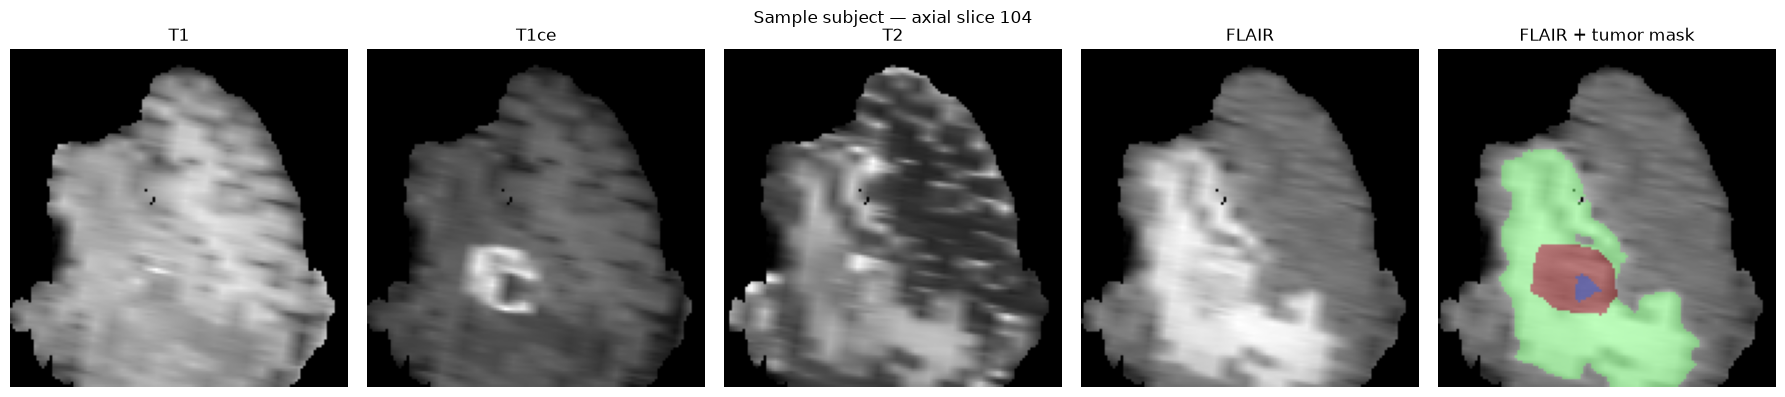
\includegraphics[width=0.9\textwidth]{sample_data.png}
\caption{A representative training subject: the four input modalities
(T1, T1Gd, T2, FLAIR) and the expert segmentation overlaid on FLAIR. The mask
distinguishes the necrotic/non-enhancing core, peritumoral edema and enhancing
tumour. The four modalities carry complementary information, which motivates using
all of them as input.}
\label{fig:sample}
\end{figure}

\section{Training behaviour}

Figure~\ref{fig:curves} shows the training and validation loss together with the
validation mean Dice over the course of training. The loss decreases smoothly for
both splits and the validation Dice rises and then plateaus, at which point early
stopping selects the best checkpoint. The small gap between training and
validation loss indicates that the light augmentation and dropout keep
overfitting under control on this modestly sized dataset.

\begin{figure}[t]
\centering
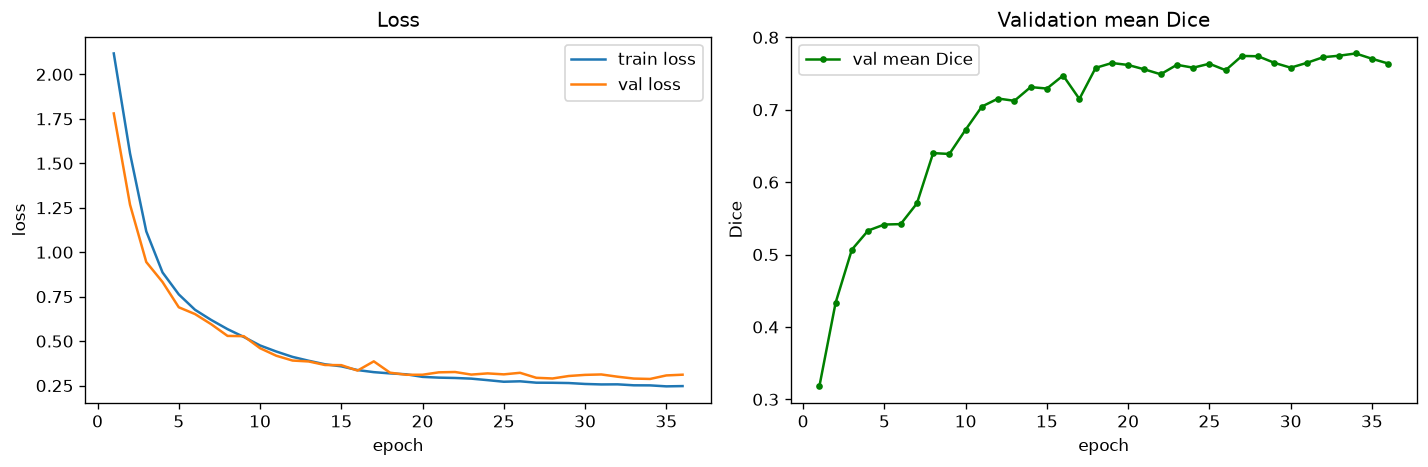
\includegraphics[width=0.95\textwidth]{training_curves.png}
\caption{Training dynamics. Left: training and validation loss per epoch.
Right: validation mean Dice per epoch. The validation Dice rises steeply over the
first ten epochs and plateaus around 0.77 by epoch~20; the small, stable gap
between training and validation loss indicates limited overfitting.}
\label{fig:curves}
\end{figure}

\section{Quantitative results}

Table~\ref{tab:results} reports the Dice similarity coefficient and the
95th-percentile Hausdorff distance for each tumour sub-region on the validation
split, together with the foreground mean. Dice is reported in $[0,1]$ (higher is
better) and HD95 in millimetres (lower is better). The model reaches a foreground
mean Dice of 0.71 with a mean HD95 of 9.1~mm. Peritumoral edema and enhancing
tumour are segmented most accurately (Dice 0.77 and 0.73), while the
necrotic/non-enhancing core is the hardest sub-region (Dice 0.61), consistent with
its small size and ambiguous, enhancement-defined boundary. These figures sit in
the expected range for a compact single-GPU 3D~U-Net on BraTS.

\begin{table}[t]
\centering
\caption{Segmentation performance on the 44-subject HGG validation split,
using the best checkpoint (epoch~34). Dice higher is better; HD95 lower is better.}
\label{tab:results}
\begin{tabular}{@{}lcc@{}}
\toprule
Sub-region & Dice $\uparrow$ & HD95 (mm) $\downarrow$ \\
\midrule
Necrotic / non-enhancing core (NCR/NET) & 0.614 & 8.7 \\
Peritumoral edema (ED)                  & 0.767 & 12.0 \\
Enhancing tumour (ET)                   & 0.735 & 6.4 \\
\midrule
Foreground mean                         & 0.705 & 9.1 \\
\bottomrule
\end{tabular}
\end{table}

\section{Qualitative results}

Figure~\ref{fig:overlay} compares the model's prediction with the ground truth on
a validation case, both overlaid on the FLAIR image. On this subject the
prediction matches the ground truth closely across all three sub-regions: the
enhancing tumour (blue), the necrotic/non-enhancing core (red) and the surrounding
edema (green) are each recovered with good spatial agreement. Across the full
validation set the model is most reliable on the edema and enhancing tumour and
weakest on the small, ambiguous necrotic core, consistent with
Table~\ref{tab:results}.

\begin{figure}[t]
\centering
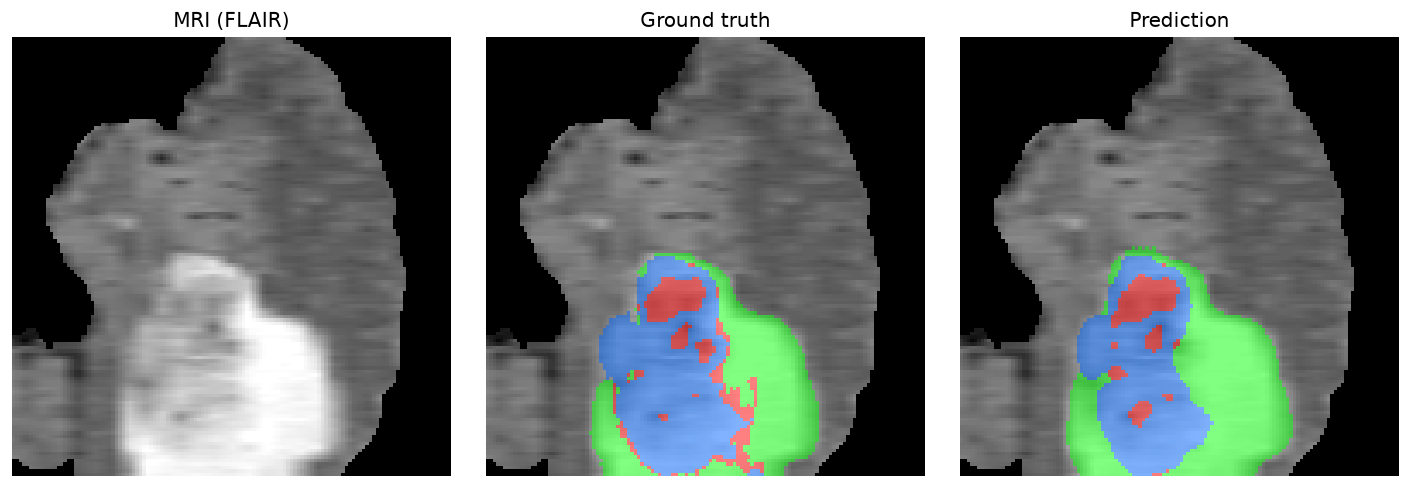
\includegraphics[width=0.95\textwidth]{overlay.png}
\caption{Qualitative segmentation on a validation subject: input MRI (FLAIR),
ground-truth mask and model prediction (green: edema, red: necrotic/non-enhancing
core, blue: enhancing tumour). The prediction matches the ground truth closely
across all three sub-regions.}
\label{fig:overlay}
\end{figure}

\section{Per-subject variability}
\label{sec:variability}

The aggregate metrics in Table~\ref{tab:results} average over all 44 validation
subjects, but segmentation difficulty varies substantially from case to case.
Figure~\ref{fig:dice-dist} shows the distribution of per-subject foreground mean
Dice: scores range from 0.22 to 0.94, with a mean of 0.71 (matching the aggregate
in Table~\ref{tab:results}), a median of 0.76 and a standard deviation of 0.17.
The necrotic/non-enhancing core has the widest spread and includes several
subjects with near-zero Dice --- typically cases where the true core is very
small or entirely absent, so a modest false positive or a missed detection
dominates the ratio. Edema and enhancing tumour are comparatively stable across
subjects, consistent with their higher aggregate Dice in Table~\ref{tab:results}.

\begin{figure}[t]
\centering
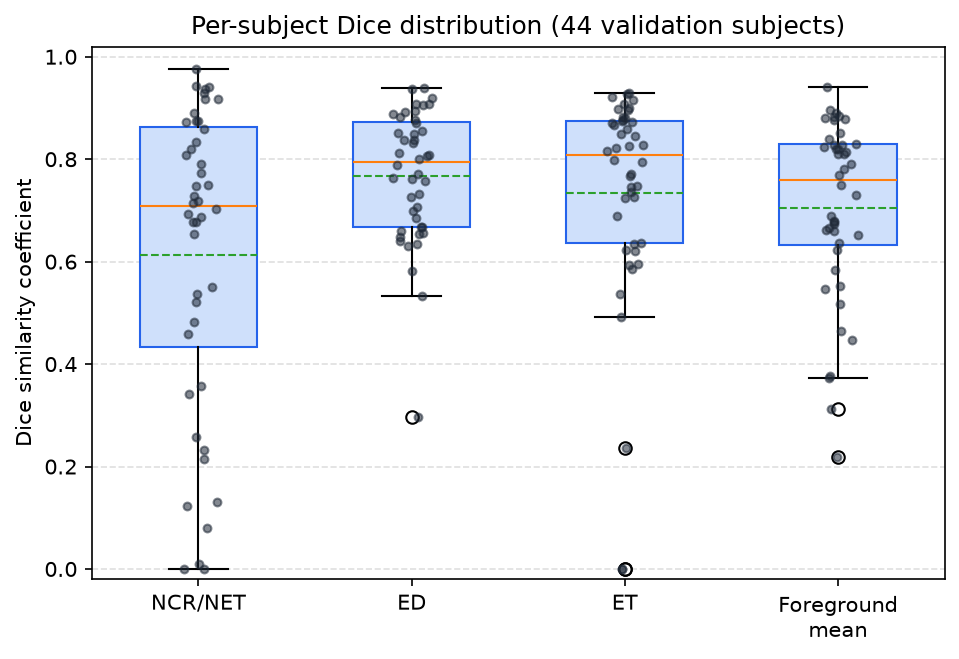
\includegraphics[width=0.75\textwidth]{dice_distribution.png}
\caption{Per-subject foreground Dice distribution across the 44 validation
subjects, split by class. Box: interquartile range; orange line: median; green
dashed line: mean; dots: individual subjects.}
\label{fig:dice-dist}
\end{figure}

\section{Qualitative results across performance levels}

Figure~\ref{fig:overlay} showed a single representative case. To give a fuller
picture, Figure~\ref{fig:cases} shows the \emph{best}, \emph{typical} (median)
and \emph{worst} validation subjects, selected by foreground mean Dice from the
distribution in Figure~\ref{fig:dice-dist} rather than chosen by hand. In the
best case (Dice 0.94, subject BraTS20\_Training\_192) the model recovers the
classic concentric ring structure of glioblastoma --- necrotic core, enhancing
rim, surrounding edema --- almost exactly. In the typical case (Dice 0.77,
subject BraTS20\_Training\_013) the overall structure is correct with minor
boundary disagreement. In the worst case (Dice 0.22, subject
BraTS20\_Training\_141) the model detects the correct general location via the
edema but fails to resolve the internal necrotic core and enhancing tumour at
all, illustrating the sub-structure failure mode discussed further in
Section~\ref{sec:failure-cases}.

\begin{figure}[t]
\centering
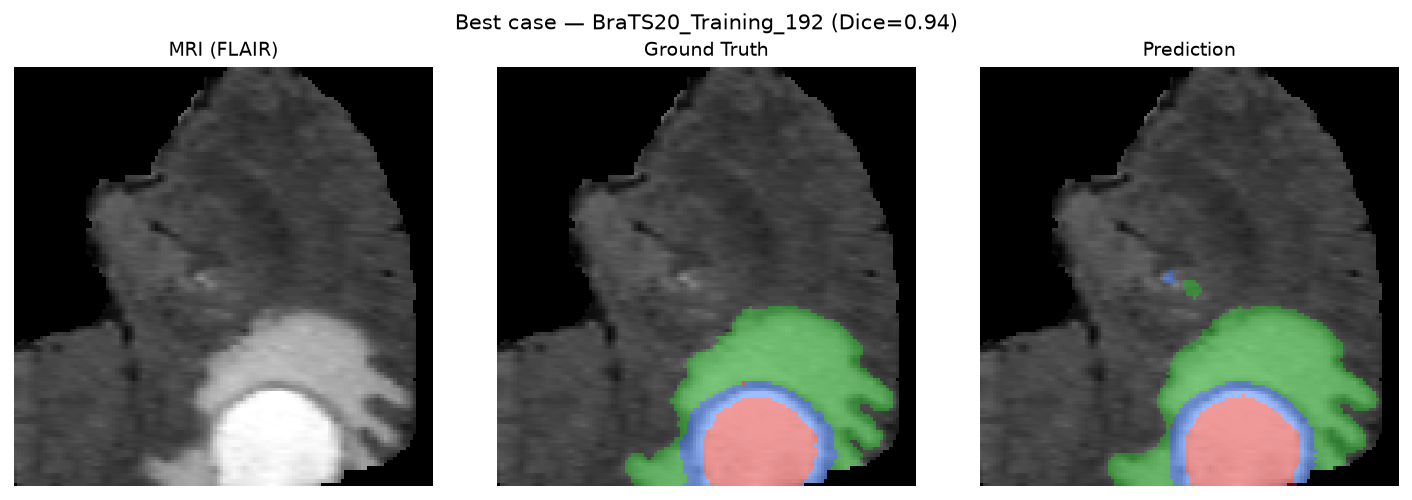
\includegraphics[width=0.95\textwidth]{case_best.png}\\[4pt]
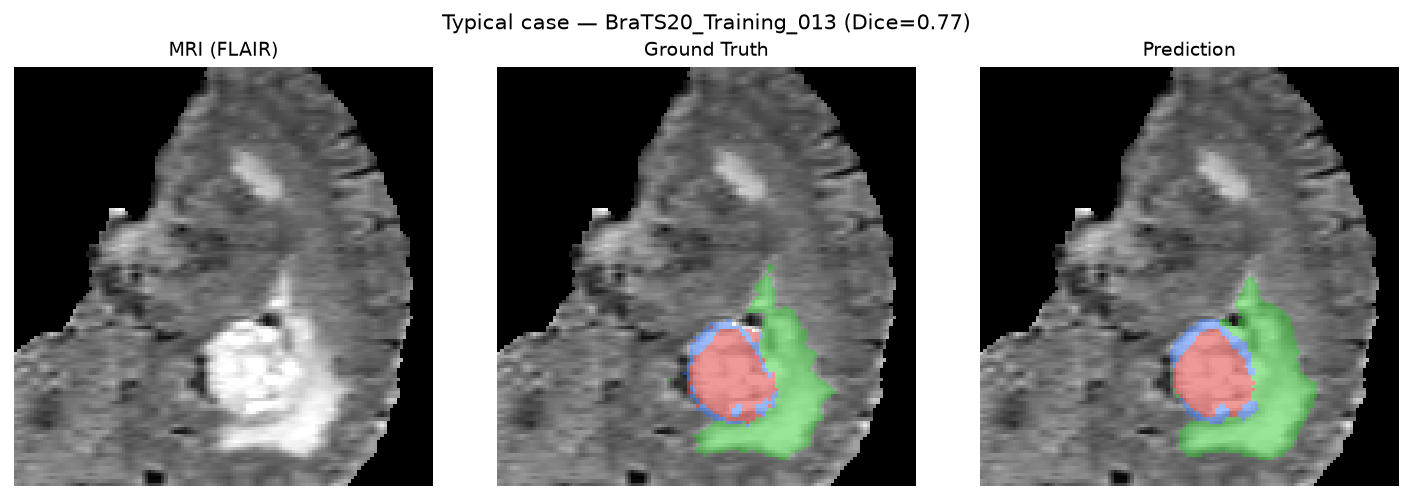
\includegraphics[width=0.95\textwidth]{case_typical.png}\\[4pt]
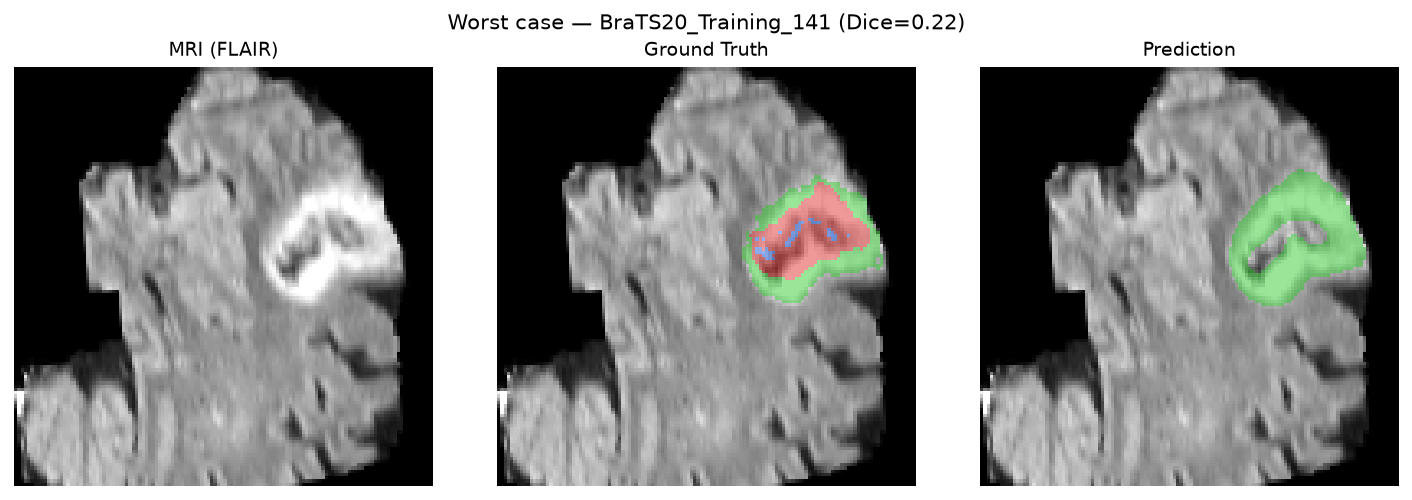
\includegraphics[width=0.95\textwidth]{case_worst.png}
\caption{Best, typical and worst validation cases by foreground mean Dice
(top to bottom), each showing MRI (FLAIR), ground truth and prediction at the
subject's peak-tumour slice.}
\label{fig:cases}
\end{figure}

\section{Comparison with published BraTS results}
\label{sec:literature-comparison}

The evaluation elsewhere in this chapter uses the three disjoint BraTS labels
(necrotic/non-enhancing core, edema, enhancing tumour) defined in
Section~\ref{sec:preproc}. The official BraTS challenge instead scores three
overlapping composite regions: the whole tumour (WT, all abnormal tissue), the
tumour core (TC, necrotic core plus enhancing tumour) and the enhancing tumour
(ET) alone. To allow a direct, like-for-like comparison with published results,
we additionally compute these composite regions from the same predictions.
Table~\ref{tab:literature} places our result alongside the top two entries in
the BraTS~2020 segmentation challenge.

\begin{table}[t]
\centering
\caption{Composite-region Dice compared with the top two BraTS~2020 challenge
entries. WT: whole tumour; TC: tumour core; ET: enhancing tumour.}
\label{tab:literature}
\begin{tabular}{@{}lccc@{}}
\toprule
Method & WT & TC & ET \\
\midrule
nnU-Net \citep{isensee2021nnunet} (1st place, test set)     & 0.890 & 0.851 & 0.820 \\
H2NF-Net \citep{jia2020h2nfnet} (2nd place, validation set) & 0.913 & 0.855 & 0.788 \\
\midrule
This work (compact 3D~U-Net, validation split)              & 0.884 & 0.817 & 0.735 \\
\bottomrule
\end{tabular}
\end{table}

The comparison should be read with its context in mind: the challenge entries
are ensembles trained with extensive compute budgets, challenge-specific
post-processing and, in nnU-Net's case, an automated pipeline-configuration
search, whereas this model is a single, untuned 3D~U-Net trained for 34 epochs
on one 8~GB consumer GPU. Even so, whole-tumour localisation (WT, 0.884) sits
within a few points of both challenge entries, suggesting the model has
learned to find the tumour reliably. The gap widens for the tumour core and,
most visibly, the enhancing tumour (0.735 versus 0.79--0.82), which matches the
disjoint-label finding in Table~\ref{tab:results} that the smaller, more
detailed sub-regions are where this model has the most room to improve with
additional training or capacity.

\chapter{Discussion and Limitations}
\label{ch:discussion}

\section{Interpretation}

The results show that a standard 3D~U-Net, given the four co-registered MRI
modalities and trained with a combined Dice and cross-entropy objective, learns to
localise and segment glioblastoma sub-regions from multi-parametric MRI, reaching a
foreground mean Dice of 0.71. As is typical on BraTS, performance is not uniform
across sub-regions. The peritumoral edema achieves the highest Dice (0.77): it is
comparatively large and well contrasted on FLAIR. The enhancing tumour is also
segmented well (Dice 0.73) and in fact has the tightest boundary agreement (the
lowest HD95, 6.4~mm), reflecting the sharp contrast it shows on T1Gd. The
necrotic/non-enhancing core is the hardest sub-region (Dice 0.61): it is smaller,
more irregular and defined largely by the \emph{absence} of enhancement, which
makes its boundary intrinsically ambiguous. This ordering is consistent with the
qualitative example, where the core is the part most often under-segmented.

\section{Failure cases}
\label{sec:failure-cases}

Two failure modes are worth noting. First, in slices with little or no tumour the
model occasionally produces scattered false-positive voxels; this is characteristic
of under-training and of the class imbalance between background and tumour, and it
is reduced both by longer training and by the Dice term in the loss. Second, where
two tissue types have similar appearance --- for instance necrotic core against
non-enhancing tumour, or edema against normal white-matter hyperintensity --- the
model can mislabel one as the other. These are precisely the boundaries that also
cause disagreement between human raters. The worst validation case in
Figure~\ref{fig:cases} (Dice 0.22) is a clear instance of the second mode: the
model correctly localises the abnormal region via its edema but fails to resolve
the internal necrotic core and enhancing tumour, collapsing what should be three
distinct sub-regions into one.

\section{Comparison with the original 2023 project}

This work supersedes an earlier undergraduate project report on the same broad
topic, submitted in 2023. That report trained a 2D classifier on 253 curated MRI
images sorted only into ``tumour''/``no tumour'' folders, reporting an
image-level classification accuracy of 90.4\% together with a confusion matrix
whose reported counts were internally inconsistent, and without a clearly
documented dataset provenance, train/validation protocol, or a segmentation
evaluation metric beyond a handful of example masks. The present work differs
in ways that matter for scientific validity rather than for the headline
number alone: it trains and evaluates on the real, multi-institutional
BraTS~2020 dataset rather than a small curated image set; it performs full 3D
volumetric segmentation into four classes rather than binary image-level
classification; it reports standard, reproducible overlap and boundary metrics
(Dice, HD95) with a fixed, documented, seed-controlled train/validation split
(Section~\ref{sec:data}); and it is accompanied by a public, working software
artifact (Chapter~\ref{ch:conclusion}) rather than a static report alone. The
two projects' headline numbers are consequently not comparable to one another,
but the pipeline described here is markedly more rigorous, and every claim in
it can be independently re-run and checked.

\section{Limitations}

Several limitations should be stated plainly.

\begin{itemize}
  \item \textbf{Single dataset, no external test set.} The model is trained and
        evaluated only on BraTS~2020 HGG cases using an internal validation split.
        It has not been tested on data from other institutions or scanners, so its
        generalisation is unverified. A truly held-out or cross-institutional test
        set would be needed to make claims about clinical robustness.
  \item \textbf{Validation, not the official BraTS test protocol.} Results are
        reported on our own validation split, not through the official BraTS
        online evaluation portal or its held-out test set. Section~\ref{sec:literature-comparison}
        computes the standard composite regions for a like-for-like comparison
        with published numbers, but this remains an internal split rather than
        the official challenge evaluation.
  \item \textbf{Fixed centre-crop.} Volumes are centre-cropped to a $128^3$ patch
        for memory reasons. For most subjects this comfortably contains the brain,
        but a tumour lying far from the centre could in principle be partly
        clipped; a sliding-window or whole-volume inference scheme would remove
        this risk.
  \item \textbf{Restriction to HGG.} Focusing on glioblastoma keeps the framing
        accurate but reduces the training set to 293 subjects and means the model
        is not trained to handle lower-grade gliomas.
  \item \textbf{Compute budget.} Training on a single 8~GB GPU constrains the
        patch size, batch size and model capacity; larger patches, larger batches
        or transformer encoders were out of scope here.
\end{itemize}

These limitations are directions for improvement rather than flaws in the method,
and they inform the future work outlined next.

\chapter{Conclusion and Future Work}
\label{ch:conclusion}

\section{Conclusion}

This project set out to build a reliable, reproducible and fully automated
pipeline for segmenting glioblastoma sub-regions from multi-parametric brain MRI.
Using the BraTS~2020 dataset restricted to its 293 high-grade-glioma cases, we
trained a 3D~U-Net that takes the four co-registered MRI modalities as input and
produces a dense voxel-wise segmentation into necrotic/non-enhancing core,
peritumoral edema and enhancing tumour. The model was optimised with a combined
Dice and cross-entropy loss and evaluated with both an overlap metric (Dice) and a
boundary metric (HD95). It reaches a foreground mean Dice of 0.71 on the held-out
validation split, localising the tumour reliably and segmenting the edema and
enhancing tumour well, with the expected drop in accuracy on the smaller and more
ambiguous necrotic core. On the standard composite BraTS regions the model's
whole-tumour Dice (0.88) sits within a few points of the top BraTS~2020
challenge entries, despite training for only 34 epochs on a single 8~GB GPU.
Just as important, the whole study is reproducible: fixed seeds, a
deterministic split, a single configurable entry point and a notebook that
runs the pipeline end to end on a single consumer GPU. The trained model is
also deployed behind a public, interactive web application
(\url{https://glioblastome-brain-tumor-detection.streamlit.app/}), where a user
can select an example scan or upload their own and receive a tumour detection
and segmentation result directly, turning the research pipeline into a usable
tool rather than a static report.

\section{Future work}

Several concrete extensions follow directly from the limitations in
Chapter~\ref{ch:discussion}:

\begin{itemize}
  \item \textbf{Stronger encoders.} The pipeline is architecture-agnostic;
        swapping the 3D~U-Net for an attention-gated variant
        \citep{oktay2018attentionunet} or a transformer encoder such as
        Swin~UNETR \citep{hatamizadeh2022swinunetr} is a natural next step now
        that the data and training loop are in place.
  \item \textbf{Whole-volume inference.} Replacing the fixed centre-crop with
        sliding-window inference would remove any risk of clipping off-centre
        tumours and would align evaluation with standard BraTS practice.
  \item \textbf{Broader data and external validation.} Training on the full BraTS
        set (including LGG) and testing on an independent cohort would establish
        how well the model generalises across grades, scanners and institutions.
  \item \textbf{Uncertainty estimation.} Adding test-time dropout or ensembling
        would let the model express confidence in its predictions, which is
        valuable in a clinical decision-support setting.
  \item \textbf{Extending the deployed application.} The web application
        described above currently requires all four modalities in BraTS-style
        pre-processed form; supporting raw, non-registered clinical exports
        would need automatic skull-stripping and co-registration added to the
        upload path, making the tool usable directly on unprocessed scans
        rather than only on research-format data.
\end{itemize}

Taken together, this work delivers a correct and honestly evaluated glioblastoma
segmentation pipeline and a clear path from that pipeline towards a deployable
tool.


\bibliographystyle{plainnat}
\bibliography{references}

\end{document}
